\chapter{Mathematical preliminaries}
\label{chap:preliminaries}

\begin{supportbox}{About this chapter}
We compress here the mathematical concepts required to follow the book. We assume prior knowledge on all these topics, focusing more on describing specific notation and giving a cohesive overview. When possible, we stress the relation between some of this material (e.g., tensors) and their implementation in practice. 
\end{supportbox}

The chapter is composed of three parts that follow sequentially from each other, starting from \textbf{linear algebra}, moving to the definition of \textbf{gradients} for $n$-dimensional objects, and finally how we can \textbf{optimize} functions by exploiting such gradients. A self-contained overview of \textbf{probability theory} is given in Appendix \ref{chap:probability_theory}, with a focus on the \textbf{maximum likelihood} principle. This chapter is full of content and definitions: bear with me for a while!


\section{Linear algebra}
\label{sec:linear_algebra}

We recall here some basic concepts from linear algebra that will be useful in the following (and to agree on a shared notation). Most of the book revolves around the idea of a \textbf{tensor}.

\begin{definition}[Tensors] \addbottle
  A \textbf{tensor} $X$ is an $n$-dimensional array of elements of the same type. We use $X \sim (s_1, s_2, \ldots, s_n)$ to quickly denote the \textbf{shape} of the tensor.
\end{definition}
%
For $n=0$ we obtain \textbf{scalars} (single values), while we have \textbf{vectors} for $n=1$, \textbf{matrices} for $n=2$, and higher-dimensional arrays otherwise. Recall that we use lowercase $x$ for scalars, lowercase bold $\mathbf{x}$ for vectors, uppercase bold $\mathbf{X}$ for matrices. Tensors in the sense described here are fundamental in deep learning because they are well suited to a massively-parallel implementation, such as using GPUs or more specialized hardware (e.g., TPUs, IPUs).

A tensor is described by the type of its elements and its \textit{shape}. Most of our discussion will be centered around tensors of floating-point values (the specific format of which we will consider later on), but they can also be defined for integers (e.g., in classification) or for strings (e.g., for text). Tensors can be \textbf{indexed} to get \textbf{slices} (subsets) of their values, and most conventions from NumPy indexing\footnote{See \url{https://numpy.org/doc/stable/user/basics.indexing.html} for a review. For readability in the book we index from $1$, not from $0$.} apply. For simple equations we use pedices: for example, for a 3-dimensional tensor $X \sim (a, b, c)$ we can write $X_i$ to denote a slice of size $(b,c)$ or $X_{ijk}$ for a single scalar. We use commas for more complex expressions, such as $X_{i, :, j:k}$ to denote a slice of size $(b, k-j)$. When necessary to avoid clutter, we use a light-gray notation:
%
\begin{equation*}
    \idx{X}{ijk}
\end{equation*}
%
to visually split the indexing part from the rest, where the argument of $\idx{\bullet}{}$ can also be an expression.

\subsection{Common vector operations}
\label{subsec:common_vector_operations}

We are mostly concerned with models that can be written as composition of differentiable operations. In fact, the majority of our models will consist of basic compositions of sums, multiplications, and some additional non-linearities such as the exponential $\exp(x)$, sines and cosines, and square roots.

Vectors $\mathbf{x} \sim (d)$ are examples of 1-dimensional tensors. Linear algebra books are concerned with distinguishing between column vectors $\mathbf{x}$ and row vectors $\mathbf{x}^\top$, and we will try to adhere to this convention as much as possible. In code this is trickier, because row and column vectors correspond to $2$-dimensional tensors of shape $(1,d)$ or $(d,1)$, which are different from $1$-dimensional tensors of shape $(d)$. This is important to keep in mind because most frameworks implement broadcasting rules\footnote{See: \url{https://numpy.org/doc/stable/user/basics.broadcasting.html}. In a nutshell, broadcasting aligns the tensors' shape from the right, and repeats a tensor whenever possible to match the two shapes.} inspired by NumPy, giving rise to non-intuitive behaviors. See Box \ref{code:broadcasting} for an example of a very common error arising in implicit broadcasting of tensors' shapes.

\begin{mypy}{An example of (probably incorrect) broadcasting, resulting in a matrix output from an elementwise operation on two vectors due to their shapes. The same result can be obtained in practically any framework (NumPy, TensorFlow, JAX, ...).}{code:broadcasting}
import torch
x = torch.randn((4, 1))  # "Column" vector
y = torch.randn((4,))    # 1-dimensional tensor
print((x + y).shape)        
# [Out]: (4,4) (because of broadcasting!)
\end{mypy}

Vectors possess their own algebra (which we call a \textbf{vector space}), in the sense that any two vectors $\mathbf{x}$ and $\mathbf{y}$ of the same shape can be linearly combined $\mathbf{z} = a\mathbf{x} + b\mathbf{y}$ to provide a third vector:
%
$$
z_i=ax_i+by_i
$$
%
If we understand a vector as a point in $d$-dimensional Euclidean space, the sum is interpreted by forming a parallelogram, while the distance of a vector from the origin is given by the Euclidean ($\ell_2$) norm:
%
$$
\lVert \mathbf{x} \rVert=\sqrt{\sum_i x_i^2}
$$
%
The squared norm $\lVert \mathbf{x} \rVert^2$ is of particular interest, as it corresponds to the sum of the elements squared. The fundamental vector operation we are interested in is the \textbf{inner product} (or \textbf{dot product}), which is given by multiplying the two vectors element-wise, and summing the resulting values.


\begin{definition}[Inner product]   \addbottle
    The inner product between two vectors $\mathbf{x}, \mathbf{y} \sim (d)$ is given by:
    \begin{equation}
            \langle \mathbf{x},\mathbf{y}\rangle=\mathbf{x}^\top\mathbf{y}=\sum_ix_iy_i
    \end{equation}
\end{definition}
%
The notation $\langle \bullet, \bullet \rangle$ is common in physics, and we use it sometimes for clarity. Importantly, the dot product between two vectors is a scalar. For example, if $\mathbf{x} = [0.1, 0, -0.3]$ and $\mathbf{y}=[-4.0, 0.05, 0.1]$:
%
\begin{equation*}
    \langle \mathbf{x}, \mathbf{y} \rangle = - 0.4 + 0 - 0.03 = - 0.43
\end{equation*}
%
A simple geometric interpretation of the dot product is given by its relation with the angle $\alpha$ between the two vectors:
%
\begin{equation}
    \mathbf{x}^\top\mathbf{y}=\lVert\mathbf{x}\rVert \lVert\mathbf{y}\rVert\cos(\alpha)
     \label{eq:dot_product_cosine}
\end{equation}
%
Hence, for two normalized vectors such that $\lVert \cdot \rVert = 1$, the dot product is equivalent to the cosine of their angle, in which case we call the dot product the \textbf{cosine similarity}. The cosine similarity $\cos(\alpha)$ oscillates between $1$ (two vectors pointing in the same direction) and $-1$ (two vectors pointing in opposite directions), with the special case of $\langle \mathbf{x}, \mathbf{y} \rangle=0$ giving rise to \textbf{orthogonal} vectors pointing in perpendicular directions. Looking at this from another direction, for two normalized vectors (having unitary norm), if we fix $\mathbf{x}$, then:
%
\begin{equation}
    \mathbf{y}^* = \argmax \;\; \langle \mathbf{x}, \mathbf{y} \rangle = \mathbf{x}
    \label{eq:maximize_dot_product}
\end{equation}
%
where $\argmax$ denotes the operation of finding the value of $\mathbf{x}$ corresponding to the highest possible value of its argument. From \eqref{eq:maximize_dot_product} we see that, to maximize the dot product, the second vector must equal the first one. This is important, because in the following chapters $\mathbf{x}$ will represent an input, while $\mathbf{w}$ will represent (adaptable) parameters, so that the dot product is maximized whenever $\mathbf{x}$ `resonates' with $\mathbf{w}$ (\textbf{template matching}).

We close with two additional observations that will be useful. First, we can write the sum of the elements of a vector as its dot product with a vector $\mathbf{1}$ composed entirely of ones:
%
$$
\langle\mathbf{x},\mathbf{1}\rangle=\sum_{i=1}^d x_i
$$
%
Second, the distance between two vectors can also be written in terms of their dot products:
%
$$
\lVert \mathbf{x} -\mathbf{y}\rVert^2 = \langle \mathbf{x},\mathbf{x}\rangle + \langle \mathbf{y},\mathbf{y}\rangle - 2 \langle \mathbf{x},\mathbf{y}\rangle
$$

The case $\mathbf{y}=\mathbf{0}$ gives us $\lVert \mathbf{x} \rVert^2 = \langle \mathbf{x}, \mathbf{x} \rangle$. Both equations can be useful when writing equations or in the code.

\subsection{Common matrix operations}

In the $2$-dimensional case we have matrices:
%
$$
\mathbf{X}=\begin{bmatrix} X_{11} & \cdots & X_{1d} \\ \vdots & \ddots & \vdots \\ X_{n1} & \cdots & X_{nd}\end{bmatrix} \sim (n,d)
$$
%
In this case we can talk about a matrix with $n$ rows and $d$ columns. Of particular importance for the following, a matrix can be understood as a \textbf{stack} of $n$ vectors $(\mathbf{x}_1, \mathbf{x}_2, \ldots, \mathbf{x}_n)$, where the stack is organized in a row-wise fashion:
%
$$
\mathbf{X} = \begin{bmatrix} \mathbf{x}_1^\top \\ \vdots \\ \mathbf{x}_n^\top \end{bmatrix}
$$
%
We say that $\mathbf{X}$ represents a \textbf{batch} of data vectors. As we will see, it is customary to define models (both mathematically and in code) to work on batched data of this kind. A fundamental operation for matrices is multiplication:

\begin{definition}[Matrix multiplication] \addbottle
Given two matrices $\mathbf{X}\sim $(a,b) and $\mathbf{Y}\sim (b,c)$, matrix multiplication $\mathbf{Z} = \mathbf{X}\mathbf{Y}$, with $\mathbf{Z} \sim (a,c)$ is defined element-wise as:
%
\begin{equation}
    Z_{ij} = \langle \mathbf{X}_i, \mathbf{Y}^\top_j \rangle
    \label{eq:matrix_multiplication}
\end{equation}
%
\noindent i.e., the element $(i,j)$ of the product is the dot product between the $i$-th row of $\mathbf{X}$ and the $j$-th column of $\mathbf{Y}$.
\end{definition}
%
 As a special case, if the second term is a vector we have a matrix-vector product:
%
\begin{equation}
\mathbf{z} = \mathbf{W}\mathbf{x}
\label{eq:matrix_vector_product}
\end{equation}
%
If we interpret $\mathbf{X}$ as a batch of vectors, matrix multiplication $\mathbf{X}\mathbf{W}^\top$ is a simple \textbf{vectorized} way of computing $n$ dot products as in \eqref{eq:matrix_vector_product}, one for each row of $\mathbf{X}$, with a single linear algebra operation. As another example, matrix multiplication of a matrix by its transpose, $\mathbf{X}\mathbf{X}^\top \sim(n,n)$, is a vectorized way to compute all possible dot products of pairs of rows of $\mathbf{X}$ simultaneously.

We close by mentioning a few additional operations on matrices that will be important. 

\begin{definition}[Hadamard multiplication]
The \textbf{Hadamard multiplication} of two matrices of the same shape is done element-wise:
%
\begin{equation*}
\idx{\mathbf{X}\odot \mathbf{Y}}{ij} = {X}_{ij}{Y}_{ij}    
\end{equation*}
\end{definition}
%
While Hadamard multiplication does not have all the interesting algebraic properties of standard matrix multiplication, it is commonly used in differentiable models for performing \textit{masking} operations (e.g., setting some elements to zero) or scaling operations. Multiplicative interactions have also become popular in some recent families of models, as we will see next.

\begin{supportbox}{On the definition of matrix multiplication}
    Why is matrix multiplication defined as \eqref{eq:matrix_multiplication} and not as Hadamard multiplication? Consider a vector $\mathbf{x}$ and some generic function $f$ defined on it. The function is said to be \textbf{linear} if $f(\alpha \mathbf{x}_1 + \beta\mathbf{x}_2) =\alpha f(\mathbf{x}_1)+\beta f(\mathbf{x}_2)$. Any such function can be represented as a matrix $\mathbf{A}$ (this can be seen by extending the two vectors in a basis representation). Then, the matrix-vector product $\mathbf{A}\mathbf{x}$ corresponds to function application, $f(\mathbf{x})=\mathbf{A}\mathbf{x}$, and matrix multiplication $\mathbf{A}\mathbf{B}$ corresponds to function composition $f \circ g$, where $(f \circ g)(\mathbf{x}) = f(g(\mathbf{x}))$ and $g(\mathbf{x})=\mathbf{B}\mathbf{x}$.
\end{supportbox}
%
Sometimes we write expressions such as $\exp(\mathbf{X})$, which are to be interpreted as \textit{element-wise} applications of the operation:
%
\begin{equation}
\idx{\exp(\mathbf{X})}{ij} = \exp({X}_{ij})
\label{eq:elementwise_matrix_exp}
\end{equation}
%
By comparison, “true” matrix exponentiation is defined for a squared matrix as:

\begin{equation}
\text{mat-exp}(\mathbf{X})=\sum_{k=0}^\infty \frac{1}{k!}\mathbf{X}^k
\label{eq:true_matrix_exp}
\end{equation}
%
Importantly, \eqref{eq:elementwise_matrix_exp} can be defined for tensors of any shape, while \eqref{eq:true_matrix_exp} is only valid for (squared) matrices. This is why all frameworks, like PyTorch, have specialized modules that collect all matrix-specific operations, such as inverses and determinants. See Box \ref{code:exp} for an example.

\begin{mypy}{Difference between the element-wise exponential of a matrix and the matrix exponential as defined in linear algebra textbooks. Specialized linear algebra operations are generally encapsulated in their own sub-package.}{code:exp}
X = torch.randn((5, 5))
X = torch.exp(X)               # Element-wise exponential
X = torch.linalg.matrix_exp(X) # Matrix exponential
\end{mypy}
%
Finally, we can write \textit{reduction} operations (sum, mean, ...) across axes without specifying lower and upper indices, in which case we assume that  the summation runs along the full axis:
%
$$
\sum_i {\mathbf{X}}_{i} = \sum_{{\color{drawred}i=1}}^{{\color{drawred}n}} {\mathbf{X}}_{i}
$$
%
In PyTorch and other frameworks, reduction operations correspond to methods having an \verb+axis+ argument:

{\small
\begin{center}\mintinline{python}{r = X.sum(axis=1)}\end{center}
}

\subsection*{Computational complexity and matrix multiplication \addteacup} 

I will use matrix multiplication to introduce the topic of \textit{complexity} of an operation.  Looking at \eqref{eq:matrix_multiplication}, we see that computing the matrix $\mathbf{Z} \sim (a,c)$ from the input arguments $\mathbf{X} \sim (a,b)$ and $\mathbf{Y} \sim (b,c)$ requires $ac$ inner products of dimension $b$ if we directly apply the definition (what we call the \textit{time} complexity), while the memory requirement for a sequential implementation is simply the size of the output matrix (what we call instead the \textit{space} complexity).

To abstract away from the specific hardware details, computer science focuses on the so-called big-$\mathcal{O}$ notation, from the German \textit{ordnung} (which stands for \textit{order} of approximation). A function $f(x)$ is said to be $\mathcal{O}(g(x))$, where we assume both inputs and outputs are non-negative, if we can find a constant $c$ and a value $x_0$ such that:
%
\begin{equation}
f(x) \le cg(x) \;\; \text{ for any } x \ge x_0
\end{equation}
%
meaning that as soon as $x$ grows sufficiently large, we can ignore all factors in our analysis outside of $g(x)$. This is called an \textbf{asymptotic} analysis. Hence, we can say that a naive implementation of matrix multiplication is $\mathcal{O}(abc)$, growing linearly with respect to all three input parameters. For two square matrices of size $(n,n)$ we say matrix multiplication is \textit{cubic} in the input dimension.

Reasoning in terms of asymptotic complexity is important (and elegant), but choosing an algorithm only in terms of big-$\mathcal{O}$ complexity does not necessarily translate to practical performance gains, which depends on many details such as what hardware is used, what parallelism is supported, and so on.\footnote{When you call a specific primitive in a linear algebra framework, such as matrix multiplication \mintinline{python}{A @ B} in PyTorch, the specific low-level implementation that is executed (the \textbf{kernel}) depends on the run-time hardware, through a process known as \textbf{dispatching}. Hence, the same code can run via a GPU kernel, a CPU kernel, a TPU kernel, etc. This is made even more complex by compilers such as XLA (\url{https://openxla.org/xla}), which can optimize code by fusing and optimizing operations with a specific target hardware in mind.} As an example, it is known that the best asymptotic algorithm for multiplying two square matrices of size $(n,n)$ scales as $\mathcal{O}(n^c)$ for a constant $c < 2.4$ \cite{coppersmith1982asymptotic}, which is much better than the cubic $\mathcal{O}(n^3)$ requirement of a naive implementation. However, these algorithms are much harder to parallelize efficiently on highly-parallel hardware such as GPUs, making them uncommon in practice.

Note that from the point of view of asymptotic complexity, having access to a parallel environment with $k$ processors has no impact, since it can only provide (at best) a constant $\frac{1}{k}$ speedup over a non-parallel implementation. In addition, asymptotic complexity does not take into consideration the time it takes to move data from one location to the other, which can become the major bottleneck in many situations.\footnote{\url{https://docs.nvidia.com/deeplearning/performance/dl-performance-gpu-background/index.html}} In these cases, we say the implementation is \textit{memory-bound} as opposed to \textit{compute-bound}. Practically, this can only be checked by running a profiler over the code. We will see that analyzing the complexity of an algorithm is far from trivial due to the interplay of asymptotic complexity and observed complexity.

\subsection{Higher-order tensor operations}

Vectors and matrices are interesting because they allow us to define a large number of operations which are undefined or complex in higher dimensions (e.g., matrix exponentials, matrix multiplication, determinants, ...). When moving to higher dimensions, most of the operations we are interested into are either batched variants of matrix operations, or specific combinations of matrix operations and reduction operations. 

As an example of the former, consider two tensors $X \sim (n,a,b)$ and $Y\sim (n,b,c)$. \textbf{Batched matrix multiplication} (BMM) is defined as:
%
\begin{equation}
\idx{\text{BMM}(X,Y)}{i} = {\mathbf{X}}_{i}{\mathbf{Y}}_{i} \sim (n, a, c)
\label{eq:bmm}
\end{equation}
%
Operations in most frameworks operate transparently on batched versions of their arguments, which are assumed like in this case to be \textit{leading dimensions} (the first dimensions). For example, batched matrix multiplication in PyTorch is the same as standard matrix multiplication, see Box \ref{code:bmm}.

\begin{mypy}{BMM in PyTorch is equivalent to standard matrix multiplication. Practically every operation is implemented to run on generically batched inputs.}{code:bmm}
X = torch.randn((4, 5, 2))
Y = torch.randn((4, 2, 3))
(torch.matmul(X, Y)).shape # Or X @ Y 
# [Out]: (4, 5, 3)
\end{mypy}
%
As an example of a reduction operation, consider two tensors $X, Y \sim (a,b,c)$. A generalized version of the dot product (GDT) can be written as:
%
$$
\text{GDT}(X,Y) =\sum_{i,j,k} \idx{X \odot Y}{ijk}
$$
%
which is simply a dot product over the `flattened' versions of its inputs. This brief overview covers most of the tensor operations we will use in the rest of the book, with additional material introduced when necessary.
%
\subsection{Einstein's notation}
%
This is an optional section that covers {\footnotesize\mintinline{python}{einsum}},\footnote{\url{https://numpy.org/doc/stable/reference/generated/numpy.einsum.html}} \addteacup a set of conventions allowing the user to specify most tensor operations with a unified syntax. Let us consider again the two examples shown before, writing down explicitly all the axes:
%
\begin{align}
\text{Batched matrix multiply:} &&& M_{ijk}=\sum_z {A}_{ijz}{B}_{izk}\label{eq:bmm_idx}\\
\text{Generalized dot product:} &&& M=\sum_i\sum_j\sum_k {X}_{ijk}{Y}_{ijk}\label{eq:gdt_idx}
\end{align}
%
In line with \textbf{Einstein’s notation},\footnote{See \url{https://en.wikipedia.org/wiki/Einstein_notation}. The notation we use is a simplified version which ignores the distinction between upper and lower indices.} we can simplify the two equations by removing the sums, under the convention that any index appearing on the right but not on the left is summed over:
%
\begin{gather}
{M}_{ijk} ={A}_{ijz}{B}_{izk} \triangleq {\color{drawred}\sum_z} \; {A}_{ijz}{B}_{izk} \label{eq:einops_1}\\
M= {X}_{ijk}{Y}_{ijk} \triangleq {\color{drawred}\sum_i\sum_j\sum_k} \; {X}_{ijk}{Y}_{ijk}
\label{eq:einops_2}
\end{gather}
%
Then, we can condense the two definitions by isolating the indices in a unique string (where the operands are now on the left):
%
\begin{itemize}
    \item ‘\textit{ijz,izk→ijk}’ (batched matrix multiply);
    \item ‘\textit{ijk,ijk→}’ (generalized dot product).
\end{itemize}
%
There is a direct one-to-one correspondence between the definitions in \eqref{eq:einops_1}-\eqref{eq:einops_2} and their simplified string definition. This is implemented in most frameworks in the {\footnotesize\verb+einsum+} operation, see Box \ref{code:einsum}.
%
\begin{mypy}{Examples of using einsum in PyTorch.}{code:einsum}
# Batched matrix multiply
M = torch.einsum('ijz,izk->ijk', A, B) 
# Generalized dot product
M = torch.einsum('ijk,ijk->', A, B)    
\end{mypy}

The advantage of this notation is that we do not need to remember the API of a framework to implement a given operation; and translating from one framework to the other is transparent because the einsum syntax is equivalent. For example, PyTorch has several matrix multiplication methods, including {\footnotesize\verb+matmul+} and {\footnotesize\verb+bmm+}, with different broadcasting rules and shape constraints, and einsum provides a uniform syntax for all of them. In addition, the einsum definition of our batched matrix multiplication is identical to, e.g., the definition in JAX, see Box \ref{code:einsum_pt}.

\begin{mypy}{Example of using einsum in JAX - compare with Box \ref{code:einsum}.}{code:einsum_pt}
M = jax.numpy.einsum('ijz,izk->ijk', A, B)
\end{mypy}
%
Working with transposed axes is also simple. For example, for $A \sim (n,a,b)$ and $B \sim (n, c, b)$, a batched multiplication of $\idx{\mathbf{A}}{i}$ times $\idx{\mathbf{B}^\top}{i}$ is obtained by switching the corresponding axes in the einsum definition:

{\footnotesize
\noindent\mintinline{python}{M = torch.einsum('ijz,ikz->ijk', A, B)}
}

\noindent Because of these reasons, einsum and its generalizations (like the popular {\footnotesize\verb+einops+}\footnote{\url{http://einops.rocks}} package) have gained a wide popularity recently.

\section{Gradients and Jacobians}
\label{sec:gradients_and_jacobians}

As the name \textit{differentiable} implies, gradients play a pivotal role in the book, by allowing us to optimize our models through semi-automatic mechanisms deriving from gradient descent. To this end, we recall here some basic definitions and concepts concerning differentiation of multi-valued functions. We focus on properties that will be essential for later, partially at the expense of mathematical precision.

\subsection{Derivatives of scalar functions}

Starting from a simple function $y=f(x)$ with a scalar input and a scalar output, its derivative is defined as follows.

\begin{definition}[Derivative]
The \textbf{derivative} of $f(x)$ is defined as:

\begin{equation}
 f'(x)= \lim_{h\rightarrow 0}\frac{f(x+h)-f(x)}{h}
\end{equation}

\end{definition}

We use a variety of notation to denote derivatives: $\partial$ will denote generically derivatives and gradients of any dimension (vectors, matrices); $\partial_x$ or $\frac{\partial}{\partial x}$ to highlight the input argument we are differentiating with respect to (when needed); while $f^\prime(x)$ is specific to scalar functions and it is sometimes called \textit{Lagrange's notation}. 

We are not concerned here about the existence of the derivative of the function (which is not guaranteed everywhere even for a continuous function), which we assume as given. We will only touch upon this point when discussing derivatives of non-smooth functions, such as $f(x) = \lvert x \rvert$ in $0$ later on in Chapter \ref{chap:automatic_differentiation}.

Derivatives of simple functions can be obtained by direct application of the definition, e.g., the derivative of a polynomial should be familiar:

\begin{align*}
\partial x^p & = \lim_{h \rightarrow 0}\frac{\eqnmarkbox[drawred]{node}{(x+h)^p} - x^p}{h} = \lim_{h\rightarrow 0} \frac{1}{h} \left( px^{p-1}h + \frac{p(p-1)}{2}x^{p-2}h^2 + \ldots + h^p   \right) \\  & = \eqnmarkbox[drawblue]{node2}{px^{p-1}} + \lim_{h\rightarrow 0} \left(\frac{p(p-1)}{2} x^{p-2}h^2 + \ldots + h^{p-1}\right) = px^{p-1}
\end{align*}
\annotate[yshift=1em]{above,right}{node}{Expandable via the binomial theorem}
\annotate[yshift=-1em]{below,right}{node2}{Independent from $h$}

Geometrically, the derivative can be understood as the slope of the tangent passing through a point, or equivalently as the best first-order approximation of the function itself in that point, as shown in Figure \ref{fig:derivative}. This is a fundamental point of view, because the slope of the line tells us how the function is evolving in a close neighborhood: for a positive slope, the function is increasing on the right and decreasing on the left (again, for a sufficiently small interval), while for a negative slope the opposite is true. As we will see, this insight extends to vector-valued functions.

\begin{SCfigure}
    \centering
    \hspace{1em}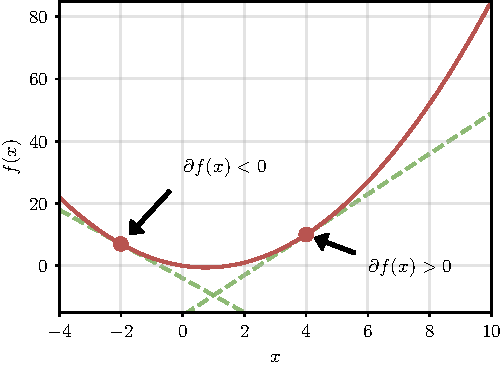
\includegraphics[width=0.6\textwidth]{images/gradient_info.pdf}
    \caption{Plot of the function $f(x)=x^2 -1.5x$, shown along with the derivatives on two separate points.}
    \label{fig:derivative}
\end{SCfigure}


We recall some important properties of derivatives that extend to the multi-dimensional case:
%
\begin{itemize}
    \item \textbf{Linearity}: the derivative is linear, so the derivative of a sum is the sum of derivatives:
    %
    $$
    \partial \Big[{\color{drawred}f(x)} + {\color{drawgreen}g(x)}\Big] = {\color{drawred}{f}^\prime(x)} + {\color{drawgreen}g^\prime(x)} \,.
    $$
    \item \textbf{Product rule}:
    %
    $$
    \partial\Big[ {\color{drawred}f(x)}{\color{drawgreen}g(x)}\Big] = {\color{drawred}{f}^\prime(x)}{\color{drawgreen}g(x)} + {\color{drawred}f(x)}{\color{drawgreen}g'(x)} \,,
    $$
    \item \textbf{Chain rule}: the derivative of function composition is given by multiplying the corresponding derivatives:
    %
    \begin{equation}
        \partial \Big[{\color{drawred}f(}{\color{drawgreen}g(x)}{\color{drawred})}\Big] = {\color{drawred}{f^\prime}(}{\color{drawgreen}g(x)}{\color{drawred})}{\color{drawgreen}g'(x)} \,
    \end{equation}
\end{itemize}

\subsection{Gradients and directional derivatives}

Consider now a function $y = f(\mathbf{x})$ taking a vector $\mathbf{x} \sim(d)$ as input. Talking about infinitesimal perturbations here does not make sense unless we specify the direction of this perturbation (while in the scalar case we only had “left” and “right”, in this case we have infinite possible directions in the Euclidean space). In the simplest case, we can consider moving along the $i$-th axis, keeping all other values fixed:
%
\begin{equation}
\partial_{x_i} f(\mathbf{x}) = \frac{\partial y}{\partial x_i} = \lim_{h \rightarrow 0} \frac{f(\mathbf{x} + h\mathbf{e}_i) - f(\mathbf{x})}{h} \,,
\label{eq:partial_derivative}
\end{equation}
%
where $\mathbf{e}_i \sim (d)$ is the $i$-th basis vector (the $i$-th row of the identity matrix):
%
\begin{equation}
\idx{\mathbf{e}_i}{j} = \begin{cases} 1 & \text{ if } i =j \\ 0 & \text{otherwise} \end{cases}
\label{eq:basis_vector}
\end{equation}
%
\eqref{eq:partial_derivative} is called a \textbf{partial derivative}. Stacking all partial derivatives together gives us a $d$-dimensional vector called the \textbf{gradient} of the function.

\begin{definition}[Gradient] \addbottle
The \textbf{gradient} of a function $y = f(\mathbf{x})$ is given by:
%
\begin{equation}
    \nabla f(\mathbf{x}) = \partial f(\mathbf{x})=\begin{bmatrix} \partial_{x_1} f(\mathbf{x}) \\ \vdots \\ \partial_{x_d} f(\mathbf{x}) \end{bmatrix}
\end{equation}
\end{definition}

Because gradients are fundamental, we use the special notation $\nabla f(\mathbf{x})$ to distinguish them. What about displacements in a general direction $\mathbf{v}$? In this case we obtain the \textbf{directional derivative}:
%
\begin{equation}
\mathrm{D}_{\mathbf{v}}f(\mathbf{x}) = \lim_{h \rightarrow 0} \frac{f(\mathbf{x} + h\mathbf{v}) - f(\mathbf{x})}{h} \,,
\label{eq:directional_derivative}
\end{equation}
%
Movement in space can be decomposed by considering individual displacements along each axis, hence it is easy to prove that the directional derivative is given by the dot product of the gradient with the displacement vector $\mathbf{v}$:
%
\begin{equation}
\mathrm{D}_\mathbf{v} f(\mathbf{x})=\langle\nabla f(\mathbf{x}),\mathbf{v}\rangle = \sum_i \eqnmarkbox[drawred]{node}{\partial_{x_i} f(\mathbf{x})v_i}
\label{eq:directional_derivative_dot_product}
\end{equation}
\annotate[yshift=-1em]{below,right}{node}{Displacement on the $i$-th axis}

Hence, knowing how to compute the gradient of a function is enough to compute all possible directional derivatives.

\subsection{Jacobians}

Let us now consider the generic case of a function $\mathbf{y} = f(\mathbf{x})$ \addclock with a vector input $\mathbf{x} \sim (d)$ as before, and this time a \textit{vector} output $\mathbf{y} \sim(o)$. As we will see, this is the most general case we need to consider. Because we have more than one output, we can compute a gradient for each output, and their stack provides an $(o, d)$ matrix we call the \textbf{Jacobian} of $f$.

\begin{definition}[Jacobian]
The \textbf{Jacobian} matrix of a function $\mathbf{y} = f(\mathbf{x})$, $\mathbf{x} \sim (d)$, $\mathbf{y} \sim (o)$ is given by:
%
\begin{equation}
\partial f(\mathbf{x}) = \begin{pmatrix}				\frac{\partial y_1}{\partial x_1} & \dots & \frac{\partial y_1}{\partial x_d} \\				\vdots & \ddots & \vdots \\				\frac{\partial y_o}{\partial x_1} & \dots & \frac{\partial y_o}{\partial x_d} \\			\end{pmatrix} \sim (o,d)
\end{equation}
\end{definition}

We recover the gradient for $o=1$, and the standard derivative for $d=o=1$. Jacobians inherit all the properties of derivatives: importantly, the Jacobian of a composition of functions is now a \textit{matrix multiplication} of the corresponding individual Jacobians:
%
\begin{equation}
\partial\left[f(g(\mathbf{x}))\right] = \left[\partial f(\bullet)\right]\partial g(\mathbf{x})
\label{eq:jacobian_chain_rule}
\end{equation}
%
where the first derivative is evaluated in $g(\mathbf{x}) \sim (h)$. See \cite[Chapter 2]{petersen2008matrix} for numerical examples of worked out gradients and Jacobians. Like in the scalar case, gradients and Jacobians can be understood as linear functions tangent to a specific point. In particular, the gradient is the best “first-order approximation” in the following sense. For a point $\mathbf{x}_0$, the best linear approximation in an infinitesimal neighborhood of $f(\mathbf{x}_0)$ is given by:

\vspace{0.5em}
$$
\widetilde{f}(\mathbf{x})= f(\mathbf{x}_0)+\langle \eqnmarkbox[drawred]{node}{\partial f(\mathbf{x}_0)}, \eqnmarkbox[drawgreen]{node2}{\mathbf{x}-\mathbf{x}_0} \rangle
$$
\annotate[yshift=1em]{above,right}{node}{Slope of the line}
\annotate[yshift=-1em]{below,right}{node2}{Displacement from $\mathbf{x}_0$}

\vspace{0.5em}
This is called \textbf{Taylor's theorem}. See Box \ref{code:taylor_approximation} and Figure \ref{fig:taylor_approximation} for a visualization in the scalar case $f(x) = x^2 - 1.5x$.

\begin{mypy}{Example of computing a first-order approximation (scalar case). The result is plotted in Figure \ref{fig:taylor_approximation}.}{code:taylor_approximation}
# Generic function
f = lambda x: x**2-1.5*x

# Derivative (computed manually for now) 
df = lambda x: 2*x-1.5 

# Linearization at 0.5 
x=0.5
f_linearized = lambda h: f(x) + df(x)*(h-x) 

# Comparing the approximation to the real derivative
print(f(x + 0.01))            # [Out]: -0.5049
print(f_linearized(x + 0.01)) # [Out]: -0.5050
\end{mypy}

\begin{SCfigure}
    \centering
    \hspace{1em}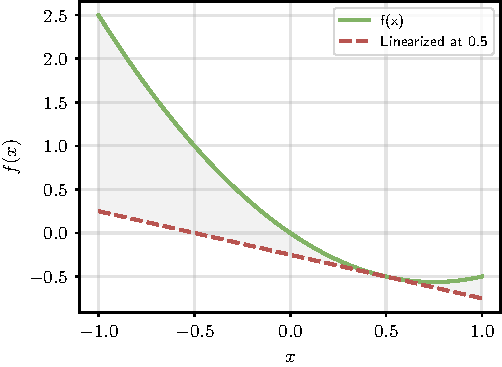
\includegraphics[width=0.6\textwidth]{images/taylor_approximation.pdf}
    \caption{The function $f(x)=x^2-1.5x$ and its first-order approximation shown in $0.5$.}
    \label{fig:taylor_approximation}
\end{SCfigure}

\subsection*{On the dimensionality of the Jacobians \addteacup}
%
We close with a pedantic note on dimensionality that will be useful in the following.   Consider the following function:
%
$$
\mathbf{y} = \mathbf{W}\mathbf{x}
$$
%
When viewed as a function of $\mathbf{x}$, the derivative is, as before, an $(o, d)$ matrix, and it can be shown that:
%
$$
\partial_{\mathbf{x}}\left[\mathbf{W}\mathbf{x}\right] =\mathbf{W}
$$
%
When viewed as a function of $\mathbf{W}$, instead, the input is itself an $(o, d)$ matrix, and the “Jacobian” in this case has shape $(o,o,d)$ (see box in the following page). However, we can always imagine an identical (isomorphic) function taking as input the vectorized version of $\mathbf{W}$, $\text{vect}(\mathbf{W})  \sim(od)$, in which case the Jacobian will be a matrix of shape $(o, od)$.

This quick example clarifies what we mean by our statement that working with vector inputs and outputs “is enough” from a notational point of view. However, it will be important to keep this point in mind in Chapter \ref{chap:automatic_differentiation}, when we will use matrix Jacobians for simplicity of notation (in particular, to avoid the proliferation of indices), but the sizes of these Jacobians may “hide” inside the actual shapes of the inputs and the outputs, most importantly the batch sizes. Importantly, we will see in Chapter \ref{chap:automatic_differentiation} that explicit computation of Jacobians can be avoided in practice by considering the so-called \textbf{vector-Jacobian products}. This can also be formalized by viewing Jacobians as abstract linear maps - see \cite{blondel2024elements} for a formal overview of this topic.

\begin{supportbox}{Working out the Jacobian}
To compute the Jacobian $\partial_{\mathbf{W}} \mathbf{W}\mathbf{x}$, we can rewrite the expression element-wise as:
%
$$
y_i=\sum_j W_{ij}x_j
$$
%
from which we immediately find that:
%
\begin{equation}
\frac{\partial y_i}{\partial W_{ij}}=x_j
\label{eq:partial_yi_wij}
\end{equation}
%
Note that to materialize the Jacobian explicitly (store it in memory), we would need a lot of repeated values. As we will see in Chapter \ref{chap:automatic_differentiation}, this can be avoided because, in practice, we only care about the application of the Jacobian on another tensor.
\label{supportbox:jacobian}
\end{supportbox}

\section{Numerical optimization and gradient descent} 

\addclock To understand the usefulness of having access to gradients, consider the problem of  minimizing a generic function $f(\mathbf{x})$, with $\mathbf{x} \sim (d)$: 
%
\begin{equation}
\mathbf{x}^* = \underset{\mathbf{x}}{\arg\min} \; f(\mathbf{x})
\label{eq:optimization}
\end{equation}
%
where, similarly to $\argmax$, $\arg\min \; f(\mathbf{x})$ denotes the operation of finding the value of $\mathbf{x}$ corresponding to the lowest possible value of $f(\mathbf{x})$. We assume the function has a single output (\textbf{single-objective optimization}), and that the domain over which we are optimizing $\mathbf{x}$ is unconstrained. 

In the rest of the book $\mathbf{x}$ will encode the parameters of our model, and $f$ will describe the performance of the model itself on our data, a setup called \textbf{supervised learning} that we introduce in the next chapter. We can consider minimizing instead of maximizing with no loss of generality, since minimizing $f(\mathbf{x})$ is equivalent to maximizing $-f(\mathbf{x})$ and vice versa (to visualize this, think of a function in 1D and rotate it across the $x$-axis, picturing what happens to its low points).

In very rare cases, we may be able to express the solution in closed-form (we will see one example in the context of least-squares optimization in Section \ref{subsec:least_squares}). In general, however, we are forced to resort to iterative procedures. Suppose we start from a random guess $\mathbf{x}_0$ and that, for every iteration, we take a step, that we decompose in terms of its magnitude $\eta_t$ (the length of the step) and the direction $\mathbf{p}_t$:

\vspace{1em}
\begin{equation}
\mathbf{x}_t = \eqnmarkbox[drawred]{node}{\mathbf{x}_{t-1}} + \eqnmarkbox[drawblue]{node2}{\eta_t\mathbf{p}_t}
\label{eq:iterative_descent}
\end{equation}
\annotate[yshift=1em]{above,right}{node}{Guess at iteration $t$}
\annotate[yshift=-1em]{below,right}{node2}{Displacement at iteration $t$}

\vspace{1em}
We call $\eta_t$ the \textbf{step size} (or, in machine learning terminology, the \textbf{learning rate}, for reasons that will become clear in the next chapter). A direction $\mathbf{p}_t$ for which there exists an $\eta_t$ such that $f(\mathbf{x}_t) \le f(\mathbf{x}_{t-1})$ is called a \textbf{descent direction}. If we can select a descent direction for every iteration, and if we are careful in the choice of step size, the iterative algorithm in \eqref{eq:iterative_descent} will converge to a minimum in a sense to be described shortly.

For differentiable functions, we can precisely quantify all descent directions by using the directional derivative from \eqref{eq:directional_derivative}, as they can be defined as the directions inducing a negative change with respect to our previous guess $\mathbf{x}_{t-1}$:
%
$$
\mathbf{p}_t \text{ is a descent direction} \;\;\Rightarrow\;\; \mathrm{D}_{\mathbf{p}_t} f(\mathbf{x}_{t-1}) \le 0
$$
%
Using what we learned in Section \ref{sec:gradients_and_jacobians} and the definition of the dot product in terms of cosine similarity from \eqref{eq:dot_product_cosine} we get:
%
$$
\mathrm{D}_{\mathbf{p}_t} f(\mathbf{x}_{t-1})=\langle \nabla f(\mathbf{x}_{t-1}), \mathbf{p}_t\rangle=\lVert\nabla f(\mathbf{x}_{t-1})\rVert \lVert\mathbf{p}_t\rVert \cos(\alpha)
$$
%
where $\alpha$ is the angle between $\mathbf{p}_t$ and $\nabla f(\mathbf{x}_{t-1})$. Considering the expression on the right, the first term is a constant with respect to $\mathbf{p}_t$. Because we have assumed $\mathbf{p}_t$ only encodes the direction of movement, we can also safely restrict it to $\lVert\mathbf{p}_t\rVert = 1$, rendering the second term another constant. Hence, by the properties of the cosine we deduce that any $\mathbf{p}_t$ whose angle is between $\pi/2$ and $3\pi/2$ with $\nabla f(\mathbf{x}_{t-1})$ is a descent direction. Among these, the direction $\mathbf{p}_t = -\nabla f(\mathbf{x}_{t-1})$ (with an angle of $\pi$) has the lowest possible directional derivative, and we refer to it as the \textbf{steepest descent direction}. 

Putting together this insight with the iterative procedure in \eqref{eq:iterative_descent} gives us an algorithm to minimize any differentiable function, that we call \textbf{(steepest) gradient descent}.

\begin{definition}[(Steepest) Gradient descent] \addbottle
Given a differentiable function $f(\mathbf{x})$, a starting point $\mathbf{x}_0$, and a step size sequence $\eta_t$, \textbf{gradient descent} proceeds as:
%
\begin{equation}
\mathbf{x}_{t}=\mathbf{x}_{t-1}-\eta_t\nabla f(\mathbf{x}_{t-1})
\label{eq:gradient_descent}
\end{equation}
\end{definition}

We will not be concerned with the problem of finding an appropriate step size, which we will just assume “small enough” so that the gradient descent iteration provides a reduction in $f$. In the next section we focus on what points are obtained by running gradient descent from a generic initialization. Note that gradient descent is as efficient as the procedure we use to compute the gradient: we introduce a general efficient algorithm to this end in Chapter \ref{chap:automatic_differentiation}.

\subsection{Convergence of gradient descent}

When discussing the convergence of gradient descent, we need to clarify what we mean by “a minimizer” of a function. If you do not care about convergence and you trust gradient descent to go well, proceed with no hesitation to the next section.

\begin{definition}[Minimum]
A \textbf{local minimum} of $f(\mathbf{x})$ is a point $\mathbf{x}^+$ such that the following is true for some $\varepsilon > 0$:
%
$$
f(\mathbf{x}^+)\le f(\mathbf{x}) \;\;\; \forall \mathbf{x} \; :\; \eqnmarkbox[drawred]{node}{\lVert \mathbf{x}-\mathbf{x}^+ \rVert <\varepsilon}
$$
\annotate[yshift=-1em]{below,left}{node}{Ball of size $\varepsilon$ centered in $\mathbf{x}^+$}

\end{definition}

In words, the value of $f(\mathbf{x}^+$) is a minimum if we consider a sufficiently small neighborhood of $\mathbf{x}^+$. Intuitively, in such a point the slope of the tangent will be $0$, and the gradient everywhere else in the neighborhood of $\mathbf{x}^+$ will point upwards. We can formalize the first idea by the concept of \textbf{stationary points}.

\begin{definition}[Stationary points]
    A \textbf{stationary point} of $f(\mathbf{x})$ is a point $\mathbf{x}^+$ such that $\nabla f(\mathbf{x}^+)=0$.
\end{definition}

Stationary points are not limited to minima: they can be maxima (the minima of $-f(\mathbf{x})$) or \textbf{saddle points}, which are inflexion points where the curvature of the function is changing (see Figure \ref{fig:saddle_point} for an example). In general, without any constraint on $f$, gradient descent can only be proven to converge to a generic stationary point depending on its initialization.

\begin{SCfigure}
    \centering
    \hspace{1em}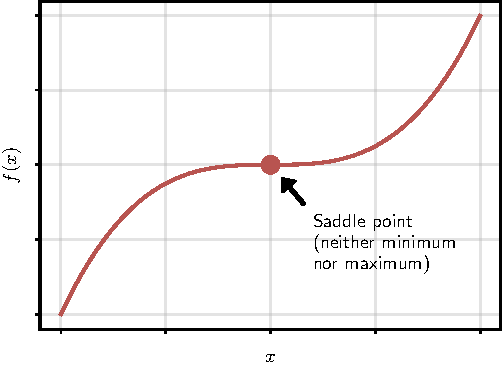
\includegraphics[width=0.6\textwidth]{images/saddle_point.pdf}
    \caption{Simple example of a saddle point (try visualizing the tangent line in that point to see it is indeed stationary).}
    \label{fig:saddle_point}
\end{SCfigure}

Can we do better? Picture a parabola: in this case, the function does not have any saddle points, and it only has a single minimum. This minimum is also special, in the sense that the function in that point attains its lowest possible value across the entire domain: we say this is a \textbf{global minimum}.

\begin{definition}[Global minimum]
    A \textbf{global minimum} of $f(\mathbf{x})$ is a point $\mathbf{x}^*$ such that $f(\mathbf{x}^*) \le f(\mathbf{x})$ for any possible input $\mathbf{x}$.
\end{definition}

Intuitively, gradient descent will converge to this global minimum if run on a parabola (from any possible initialization) because all gradients will point towards it. We can generalize this idea with the concept of \textbf{convexity} of a function. There are many possible definitions of convexity, we choose the one below for simplicity of exposition.

\begin{definition}[Convex function]
    A function $f(\mathbf{x})$ is convex if for any two points $\mathbf{x}_1$ and $\mathbf{x}_2$ and $\alpha \in \left[0,1\right]$ we have:

    \vspace{1em}
    \begin{equation}
        f(\eqnmarkbox[drawblue]{node}{\alpha \mathbf{x}_1 + (1-\alpha)\mathbf{x}_2})\le \eqnmarkbox[drawred]{node2}{\alpha f(\mathbf{x}_1)+(1-\alpha)f(\mathbf{x}_2)}
        \label{eq:convex_function}
    \end{equation}
    \annotate[yshift=-1em]{below,right}{node}{Interval from $\mathbf{x}_1$ to $\mathbf{x}_2$}
    \annotate[yshift=1em]{above,right}{node2}{Line segment from $f(\mathbf{x}_1)$ to $f(\mathbf{x}_2)$}
\end{definition}

\vspace{1em}
The left-hand side in \eqref{eq:convex_function} is the value of $f$ on any point inside the interval ranging from $\mathbf{x}_1$ to $\mathbf{x}_2$, while the right-hand side is the corresponding value on a line connecting $f(\mathbf{x}_1)$ and $f(\mathbf{x}_2)$. If the function is always below the line joining any two points, it is convex (as an example, a parabola pointing upwards is convex). 

Convexity qualifies the simplicity of optimizing the function, in the following sense \cite{jain2017non}:
%
\begin{enumerate}
    \item For a generic \textit{non-convex} function, gradient descent converges to a \textit{stationary point}. Nothing more can be said unless we look at higher-order derivatives (derivatives of the derivatives).
    \item For a \textit{convex} function, gradient descent will converge to a \textit{global minimum}, irrespective of initialization.
    \item  If the inequality in \eqref{eq:convex_function} is satisfied in a strict way (\textbf{strict convexity}), the global minimizer will also be \textit{unique}.
\end{enumerate}

This is a hard property: to find a global minimum in a non-convex problem with gradient descent, the only solution is to run the optimizer infinite times from any possible initialization, turning it into an NP-hard task \cite{jain2017non}.

This discussion has a strong historical significance. As we will see in Chapter \ref{chap:fully_connected_models}, any non-trivial model is non-convex, meaning that its optimization problem may have several stationary points. This is in contrast to alternative algorithms for supervised learning, such as support vector machines, which maintain non-linearity while allowing for convex optimization. Interestingly, complex differentiable models seem to work well even in the face of such restriction, in the sense that their optimization, when started from a reasonable initialization, converge to points with good empirical performance.

\subsection{Accelerating gradient descent}
The negative gradient describes the direction of steepest descent, but only in an infinitesimally small neighborhood of the point. As we will see in Chapter \ref{chap:deep_cnns} (where we introduce stochastic optimization), these directions can be extremely noisy, especially when dealing with large models. A variety of techniques have been developed to accelerate convergence of the optimization algorithm by selecting better descent directions. For computational reasons, we are especially interested in methods that do not require higher-order derivatives (e.g., the Hessian), or multiple calls to the function.

We describe here one such technique, \textbf{momentum}, and we refer to \cite[Chapter 12]{zhang2023dive}, for a broader introduction.\footnote{See also this 2016 blog post by S. Ruder: \url{https://www.ruder.io/optimizing-gradient-descent/}.} If you picture gradient descent as a ball “rolling down a hill”, the movement is relatively erratic, because each gradient can point in a completely different direction (in fact, for a perfect choice of step size and a convex loss function, any two gradients in subsequent iterations will be orthogonal). We can smooth this behavior by introducing a “momentum” term that conserves some direction from the previous gradient iteration:

\begin{align*}
\mathbf{g}_t& =- \eqnmarkbox[drawred]{node}{\eta_t\nabla f(\mathbf{x}_{t-1})} + \eqnmarkbox[drawblue]{node2}{\lambda\mathbf{g}_{t-1}} \\ 
\mathbf{x}_{t}& =\mathbf{x}_{t-1}+\mathbf{g}_t
\end{align*}
\annotate[yshift=1em]{above,right}{node}{Normal gradient descent iteration}
\annotate[yshift=-1em]{below,right}{node2}{Additional momentum term}

where we initialize $\mathbf{g}_0 = \mathbf{0}$. See Figure \ref{fig:momentum} for an example. 

\begin{SCfigure}
    \centering
    \hspace{1em}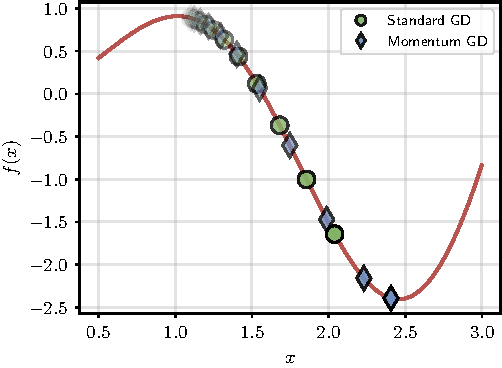
\includegraphics[width=0.6\textwidth]{images/momentum.pdf}
    \caption{First iterations of standard GD and GD with momentum when minimizing $f(x)=x\sin(2x)$ starting from $x=1+\varepsilon$, with $\lambda=0.3$.}
    \label{fig:momentum}
\end{SCfigure}

The coefficient $\lambda$ determines how much the previous term is dampened. In fact, unrolling two terms:
%
\begin{gather*}
\mathbf{g}_t=-\eta_t\nabla f(\mathbf{x}_{t-1}) +\lambda(-\eta_t\nabla f(\mathbf{x}_{t-2}) +\lambda\mathbf{g}_{t-2}) \\ = -\eta_t\nabla f(\mathbf{x}_{t-1}) -\lambda\eta_t\nabla f(\mathbf{x}_{t-2}) +\lambda^2\mathbf{g}_{t-2}
\end{gather*}
%
Generalizing, the iteration at time $t-n$ gets dampened by a factor $\lambda^{n-1}$. Momentum can be shown to accelerate training by smoothing the optimization path \cite{sutskever2013importance}. Another common technique is adapting the step size for each parameter based on the gradients’ magnitude \cite{zhang2023dive}. A common optimization algorithm combining several of these ideas is Adam \cite{kingma2014adam}. One advantage of Adam is that it is found to be relatively robust to the choice of its \textbf{hyper-parameters},\footnote{A hyper-parameter is a parameter which is selected by the user, as opposed to being learnt by gradient descent.} with the default choice in most frameworks being a good starting point in the majority of cases.

One disadvantage of using accelerated optimization algorithms can be increased storage requirements: for example, momentum requires us to store the previous gradient iteration in memory, doubling the space needed by the optimization algorithm (although in most cases, the memory required to compute the gradient is the most influential factor in terms of memory, as we will see in Section \ref{sec:reverse_mode_automatic_differentiation}).

\newpage
\section*{From theory to practice}

\begin{supportbox}{About the exercises}
This book does not have classical end-of-chapter exercises, which are covered in many existing textbooks. By contrast, I describe a self-learning path to help you explore two frameworks (JAX and PyTorch) as you progress in the book. Solutions to the more practical exercises will be published on the book's website.\footnote{\url{https://www.sscardapane.it/alice-book}} These sections are full of URLs linking to online material -- they might be expired or moved by the time you search for them.
\end{supportbox}

\subsection*{Starting from the basics: NumPy}

\begin{wrapfigure}{R}{3.0cm}
\vspace{-4em}
\includegraphics[width=3.0cm]{images/shutterstock_2075221579.jpg}
\vspace{-2em}
\end{wrapfigure} 

The starting block for any designer of differentiable models is a careful study of NumPy. NumPy implements a generic set of functions to manipulate multidimensional arrays (what we call \textit{tensors} in the book), as long as functions to index and transform their content. You can read more on the library's quick start.\footnote{\url{https://numpy.org/doc/stable/user/quickstart.html}} You should feel comfortable in handling arrays in NumPy, most notably for their indexing: the {\footnotesize\verb+rougier/numpy-100+}\footnote{\url{https://github.com/rougier/numpy-100}} repository provides a nice, slow-paced series of exercises to test your knowledge.

\subsection*{Moving to a realistic framework}

Despite its influence, NumPy is limited, in particular in his support for parallel hardware such as GPUs (unless additional libraries are used), and for his lack of automatic differentiation (introduced in Chapter \ref{chap:automatic_differentiation}). JAX replicates the NumPy's interface while adding extended hardware support, the automatic computation of gradients, and additional transformations such as the \textbf{vectorized map} (\mintinline{python}{jax.vmap}). Frameworks such as PyTorch also implement a NumPy-like interface at their core, but they make minor adjustments in nomenclature and functionality and they add several high-level utilities for building differentiable models. For the purposes of this chapter, you can skim the documentation of \mintinline{python}{jax.numpy.array} and \mintinline{python}{torch.tensor} to understand how much they have in common with NumPy. For now, you can ignore high-level modules such as \mintinline{python}{torch.nn}. We will have more to say about how these frameworks are designed in Chapter \ref{chap:automatic_differentiation}, after we introduce their gradient computation mechanism.

\subsection*{Implementing a gradient descent algorithm}

To become proficient with all three frameworks (NumPy, JAX, PyTorch), I suggest to replicate the exercise below thrice -- each variant should only take a few minutes if you know the syntax.  Consider a 2D function $f(\mathbf{x})$, $\mathbf{x} \sim (2)$, where we take the domain to be $[0,10]$:\footnote{I asked ChatGPT to generate a nice function with several minima and maxima. Nothing else in the book is LLM-generated, which I feel is becoming an important disclaimer to make.}
%
\begin{equation*}
    f(\mathbf{x}) = \sin(x_1) \cos(x_2) + \sin(0.5x_1) \cos(0.5x_2)
\end{equation*}
%
Before proceeding in the book, repeat this for each framework:
%
\begin{enumerate}
\item Implement the function in a \textbf{vectorized} way, i.e., given a matrix $\mathbf{X} \sim (n,2)$ of $n$ inputs, it should return a vector $f(\mathbf{X}) \sim (n)$ where $\idx{f(\mathbf{X})}{i} = f(\mathbf{X}_i)$.
\item Implement another function to compute its gradient (hard-coded -- we have not touched automatic differentiation yet).
\item Write a basic gradient descent procedure and visualize the paths taken by the optimization process from multiple starting points.
\item Try adding a momentum term and visualizing the norm of the gradients, which should converge to zero as the algorithm moves towards a stationary point.
\end{enumerate}
%
If you are using JAX or PyTorch to solve the exercise, point (3) is a good place to experiment with \mintinline{python}{vmap} for vectorizing a function.